% !Mode:: "TeX:UTF-8"

%除了通用系统的多核调度外,在各个特殊领域,如DSP系统、分布式计算、实时系统中,也对多任务多核的并行调度提出了各自的要求。DSP系统是传统的并行处理系统,其为了数据的最大吞吐率,往往要设计各处理单元间协同工作,哪些任务需要并行,哪些任务安排在相同或不同的处理器,哪些任务先执行,数据通路如何安排都需要精心设计。与之相比,分布式计算往往更注重通信方面的开销,其计算系统各运算单元间通信的不确定性,也为任务调度安排带来了新的变数。

%在 DSP 系统方面,现有算法能够较好的处理任务间的偏序关系,但 DSP 的调度算法主要是数据驱动型的,它对以强烈时间属性为特性的实时任务仍然难以满足需求。在分布式计算方面,主要关注点在于任务间通信以及总的调度长度,同样缺少调度算法对任务的时间要求给予特别的保证。


\chapter{相关技术介绍}

\section{实时调度算法背景简介}

%\subsection{实时调度算法}

%\emph{TODO: 调整格式、补全引用}

\subsection{任务模型}

一个基本的实时任务模型包括以下三类任务:
\begin{description}
  \item[周期性任务 (periodical)] 包括以下参数:\\
    周期 T;最坏执行时间 C;首次执行偏移 O;相对时间限 D。
  \item[偶发性任务 (sporadic)] 相比周期性任务,它的周期不是一定的,但有一个最小间隔时间。
  \item[非周期任务 (aperiodic)] 只释放一次的任务。
\end{description}

\subsection{任务的时间限}

周期性任务的时间限有以下三种分类:
\begin{itemize}
  \item 隐性时间限(implicit-deadline),任务的时间限与任务的释放周期相等。
  \item 限制时间限(constrained-deadline),每个任务的时间限都不长于它的释放周期。
  \item 任意时间限(arbitrary-deadline),时间限与释放周期无关。
\end{itemize}

大部分任务系统允许任务被抢占,并在以后被恢复且无额外开销。

一个周期性任务或偶发性任务的占用率(utilization)定义为
\begin{equation}
  U(t) = C/T
\end{equation}

一个由周期性任务和偶发性任务组成的任务系统的总占用率为各任务占用率之和。
以上任务模型根据实际因素会加入 非抢占约束、优先关系约束、互斥关系约束等。

%================================
\subsection{调度环境}

\subsubsection{离线调度}

离线调度也称为静态调度,所有任务的执行时间都认为是最坏情况的执行时间。由于任务的周期性,整体调度也是周期性的,其周期长度等于各任务周期的最小公倍数。因此,随着任务数量的增长,静态调度表的长度具有指数级的大小,对一些嵌入式系统的实现来说可能成为问题。

大部分实时系统内核实现基于优先级的调度器,分为静态优先级和动态优先级。静态优先级,每个任务被赋予一个固定,且与其他任务不同的优先级;动态优先级则在任务执行时多次重复计算。运行时调度选择最高优先级的任务执行。
一个调度算法是最优的,是指如果一个可行调度存在,该算法一定能找到可行调度。

在离线调度中,设计调度算法和检测调度可行性是同一个问题。调度算法根据任务的时间限得到一个可行调度序列。

\subsubsection{在线调度}

除了以上离线调度的情况外,基于优先级的在线调度需要考虑优先级反转现象(priority inversion phenomenon)。如果高优先级的任务 Tc 需要一个低优先级任务 Ta 的资源,而 Ta 根据优先级规则又被一个中等优先级的任务 Tb 抢占,造成 Tb 阻塞 Tc 执行的现象。调度非抢占式的任务,或者任务间需要通过网络传递消息时也会产生此现象。

在在线调度中,实时调度理论集中于以下两个问题:
\begin{itemize}
  \item 调度可行性分析:给定一个任务系统,和一个调度环境,确定是否存在一个调度满足所有时间限。
  \item 运行时调度问题:给定一个可行的任务系统,根据调度环境,确定一个调度算法能够找到满足所有时间限的调度。
\end{itemize}

%================================
\subsection{单处理器调度}

\subsubsection{动态优先级调度}

在可抢占式的单处理器调度环境下,EDF 是最优调度。即针对一个相互独立的任务集,如果存在一个可行的抢占式调度满足所有时间限,则 EDF 也能够产生满足所有时间限的抢占式调度。

LLF 是另一种动态优先级的最优调度。最小松驰时间的任务具有最高优先级。


\subsubsection{静态优先级调度}

静态优先级调度中每个任务要赋予一个与其他任务不同的优先级,而相同任务的每次执行都有相同的优先级。因此静态优先级调度问题本质上转化为给不同任务分配优先级的问题。

对隐性时间限 同步周期性任务来说,RM 调度是最优的。优先级与任务周期成反比关系。也即是说如果存在一种静态优先级分配,能够使所有任务满足时间限,那么 RM 的优先级分配也能够产生满足所有时间限的调度。

对隐性时间限 非同步的周期性任务来说,RM 被证明不是最优的优先级分配方案。

对限制时间限同步周期性任务集,DM 优先级分配是最优的。

对限制时间限非同步周期性任务集,寻找最优静态优先级的计算复杂度仍是一个待解决的问题。

%=================================
\subsection{多处理器调度}

对于周期性与偶发模型的任务调度问题来说,大部分多处理器调度假设所有任务是可抢占的,处理器间迁移也是允许的。

\subsubsection{多处理器平台}

分为同构多处理器,和一致性多处理器。同构多处理器上所有处理器完全相同,一致性多处理器上,每个处理器的运算能力是 k 倍形式的。

\subsubsection{调度算法分类}

多处理器调度主要考虑两个问题:
\begin{enumerate}
  \item 任务分配问题:任务分配给哪个处理器执行。根据分配方式,可将调度算法分为如下三类:
      \begin{itemize}
        \item 非迁移的。每个任务只能在同一个处理器上运行(也称为 partitioned 调度或分区调度)
        \item task-level 迁移。同一任务可在多个处理器上执行,但每次执行只能在一个处理器上
        \item job-level 迁移。每次执行的任务也可以执行一半后迁移到其他处理器,但不允许并行执行多份。(也称为 global 调度或全局调度)
      \end{itemize}
  \item 执行顺序问题:各处理器上任务的执行顺序及时间。同样可分为三类:
      \begin{itemize}
        \item 固定 task 优先级。如 RM 类算法
        \item 固定 job 优先级。如 EDF 类算法
        \item 动态优先级。如 LLF 类算法
      \end{itemize}
\end{enumerate}

%------------------------
多处理器的调度根据是否允许任务的迁移,主要分为分区调度(partitioned)和全局调度(global)两类。分区调度是非迁移的,即每个任务只能在同一个处理器上运行;全局调度则是允许 job-level 迁移的,即每次执行的任务可以执行一半后迁移到其他处理器继续执行。

分区调度的优势在于:
\begin{itemize}
  \item 如果一个任务运行时超出了最坏执行时间,它只影响同一处理器中的其他任务。
  \item 每个任务只运行于一个处理器上,没有迁移开销。
  \item 分区调度在每个处理器上使用一个单独的任务队列,而不像全局调度使用一整个全局队列。对于较大规模的系统,单一全局队列的开销非常巨大。
\end{itemize}

从实用角度讲,只要将任务分配到各处理器后,就可以有效利用现有单处理器调度算法的各种技术。如对隐性时间限的抢占式周期任务的静态优先级的最优调度RM;对限制时间限周期任务的静态优先级的最优调度DM;对任意时间限的抢占式偶发性任务集的最优调度 EDF。

分区调度的最大劣势是 将任务分配到不同处理器上去类似于一个打包分配问题,而这是 NP-Hard 的。

相对的,全局调度的优势在于:
\begin{itemize}
  \item 全局调度相比分区调度有更少的上下文交换/抢占开销。因为调度器只有当没有处理器空闲时才会允许任务抢占。
  \item 当任务执行时间短于其最坏执行时间时,这段时间可被用于全局的其他任务,而不只是给在同一分区的其他任务。
  \item 当有任务超过了其最坏执行时间,对整个系统来说,有更低的概率造成整个系统不满足时间限。在所有任务运行最坏执行时间的情况下,相比单处理器 全局调度更不容易造成多处理器超过时间限。
  \item 全局调度更适合于开放系统,当任务集发生改变时,不需要运行负载平衡、任务分配的算法。
\end{itemize}

大多数研究全局调度的算法都集中于允许 job-level 迁移的方法。

\subsubsection{带有约束条件的调度}

以上讨论的大部分分区及全局调度算法都仅仅针对简单的周期性和偶发性任务模型,任务的执行之间都是相互独立的。除此之外,还有一些算法考虑了任务之间对处理器以外的共享资源的互斥访问造成的阻塞,打破了任务间完全独立的假设\upcite{SurveyHRT}。


\section{多核系统计算模型}
\label{basic-MoC}

在 DSP 系统中,由于程序对大数据量吞吐率的要求,它的任务多采用静态调度,它的并行调度算法也较好的解决了任务间的数据传输、依赖关系等问题。在设计流式程序时,如何有效表达程序中的并行性是所要面对的一个挑战\upcite{Challenge}。而基于计算模型 (Model-of-Computation, MoC) 的设计则成为了解决这一挑战的事实标准\upcite{MoCdefacto}。在基于 MoC 的设计中,任务可被映射为一个有向图,图中顶点表示 运算单元(如任务),边表示通信路径。不同的 MoC 模型在 运算单元 的计算和通信方面定义不同的规则和语义。基于 MoC 的设计优势在于,显式表达了程序各部分之间的并行性等重要属性,加强了程序在设计时对运行效率的可分析性。

\subsection{几种计算模型}

在 V. Zadrija 的报告\upcite{MoCSurvey}中,分析比较了几种不同的 MoC。根据运算单元粒度的不同,MoC 可以分为面向进程的 (process-oriented) 和面向状态的 (state-oriented) 两大类。面向进程的计算模型通过并行进程间的通信来描述系统行为,其中通信方式包括消息传递或共享内存等。面向进程的计算模型强调清晰描述进程间的并行性,因此适合于在多核平台上实现,因为多核平台内在要求并行性。面向状态的计算模型通过状态机来描述系统行为,其中状态机由一个状态的集合以及转换条件构成。一般来说,状态多用来明确表示程序的内存状态。与面向进程的计算模型不同,面向状态的计算模型典型的用途是硬件实现层或者用于控制占主导的程序中。

\subsubsection{面向进程的计算模型}
在面向进程的计算模型中,一些应用最广泛的模型包括进程网络 (process networks)、 数据流模型 (dataflow models) 和进程微分 (process calculi),有时也称作进程代数 (process algebra)。
进程网络是最常见面向进程的计算模型的例子。进程网络由一系列并行的进程所组成,进程间通过缓冲区来通信,通信在发送端是异步的,数据在缓冲区中累积,而在接收端,进程一般是阻塞的,直到缓冲区中达到运行所需的最小数据才可执行。
数据流模型强化了图在表达系统行为时的作用,它用一个有向图来表示进程间的关系。与进程网络不同的是,数据流中的一个运算单元表示执行的一个原子块,从而上下文切换操作可以被避免。

% SDF 方法\upcite{SDF1987,SDF_C} 即是一种在 DSP 中使用广泛的计算模型,它能够较好的表述任务间的数据传输、依赖关系等,并由此得到有效的静态调度表。

Kahn 进程网络 (Kahn process networks, KPN)\upcite{KPN74} 是一种面向进程的计算模型,如图\ref{basic-fig-KPN} 所示。在 KPN 模型中,进程之间相互独立且并行执行,通信通过一个单向的点到点消息传递通道实现。消息传递通道与缓冲区一起,使得发送消息的进程可以异步执行。KPN 模型是适用于多核平台的计算模型,但其没有明确表述进程之间具体的数据传输量,也无法确定各进程何时可以执行,何时由于数据不足应当阻塞,也无法确定具体的缓冲区使用量,因此该模型只能用于动态调度。

\begin{figure}[!bt]
  \centering
  % Requires \usepackage{graphicx}
  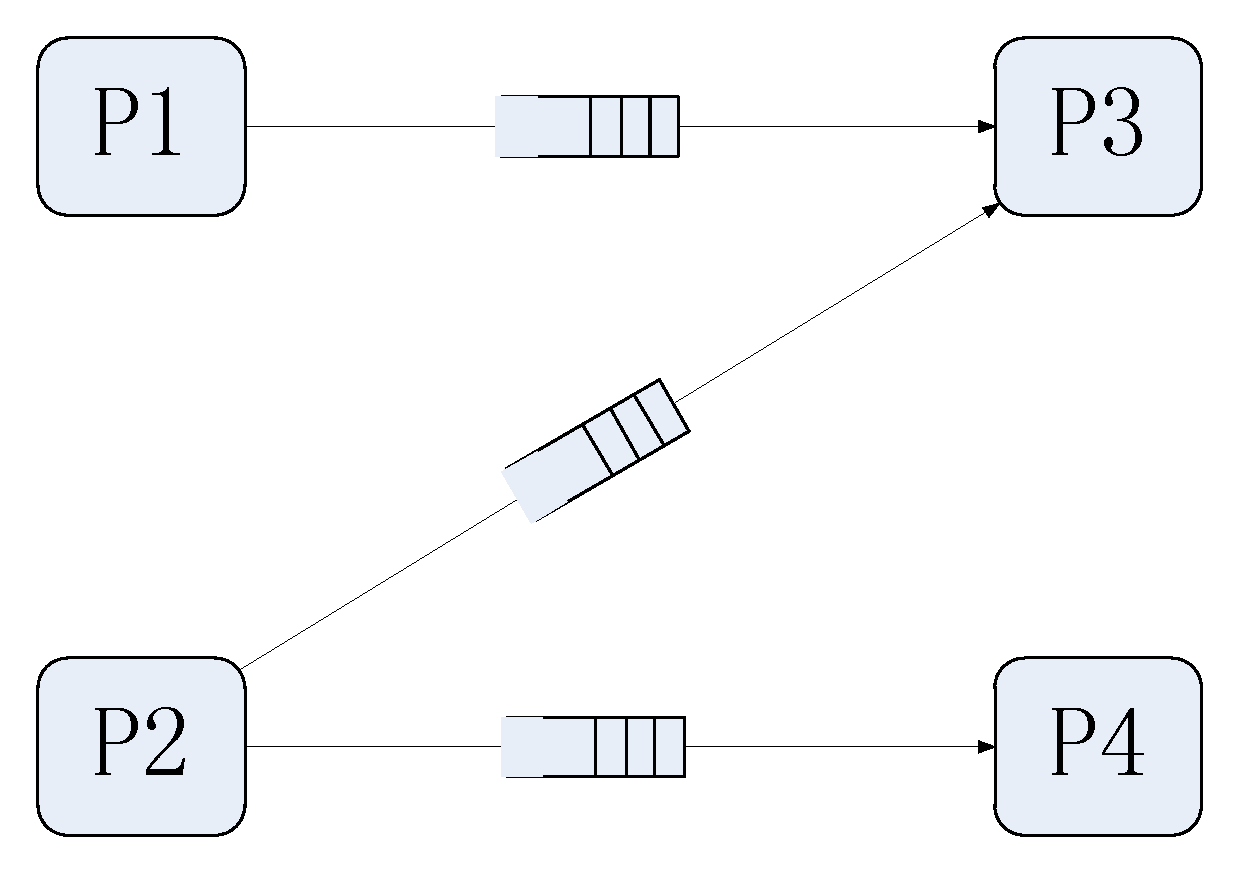
\includegraphics[height=20ex]{figure/basic-KPN.pdf}\\
  \caption{KPN 模型的例子}\label{basic-fig-KPN}
\end{figure}

同步数据流 (Synchronous Data Flow, SDF)\upcite{SDF1987} 是数据流模型的一种,在此模型中,运算单元每次执行时消耗与产生的数据量事先已知,因此系统执行时是可确定的,因此适用于静态调度,下一节将详细介绍。

此外,进程代数模型对进程之间的交互、同步通信机制提供了高层的形式化描述方法,此模型适用于分析、等价检查以及形式化验证。

\subsubsection{面向状态的计算模型}
在面向状态的计算模型中,具有代表性的几个模型有有限状态机 (finite state machines, FSM)、带数据的有限状态机 (finite state machines with data, FSMD) 等。此外,程序状态机 (Program State Machines, PSM) 可被视为一种组合了面向过程和面向状态两种类型的计算模型。这类模型多用于硬件实现层或者用于控制占主导的程序中,是动态调度的,在我们的算法中并不适合。


\subsection{SDF简介}
\label{SDF-intro}
% 简介 SDF 方法

%根据以上问题描述,以往的多核实时调度算法都不能很好的处理任务间数据依赖的约束,而DSP 中的SDF (Synchronous Data Flow)方法可以较好的描述任务间的数据依赖关系,因此可考虑用SDF的方法来解决以上问题。但SDF 方法不含有对实时任务时间约束的保证,因此需要对此方法加以改进。
在信号处理系统中,LGDF(Large grain data flow)用来表示DSP各计算单元间的数据流通。LGDF 是一个有向图,每个结点表示一个运算过程,可以是很小的运算单元,如加法器或乘法器,也可以是复杂的一段程序,如数字过滤器或FFT单元等。SDF来源于LGDF,但与之不同的是,SDF 要求每个运算单元的数据率在编译时是已知的,其中每条弧的起点表示数据出发结点一次运算所产生的数据,每条弧的终点表示数据接收结点每次运算所消耗的数据,如图\ref{basic-SDF-sample}。

\begin{figure}[!htb]
  \centering
  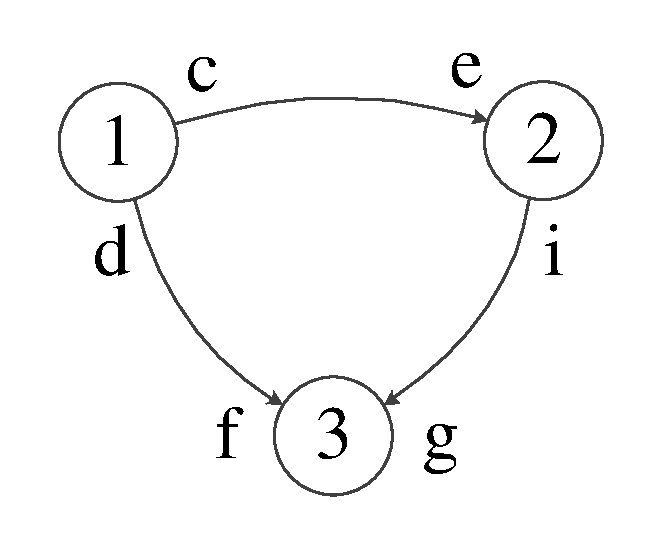
\includegraphics[height=15ex]{figure/basic-1-SDF.pdf}
  \caption{SDF图示例}
  \label{basic-SDF-sample}
\end{figure}

%\begin{figure}[!tb]
%\begin{floatrow}
%  {\ffigbox{\caption{SDF图示例}\label{basic-SDF-sample}} {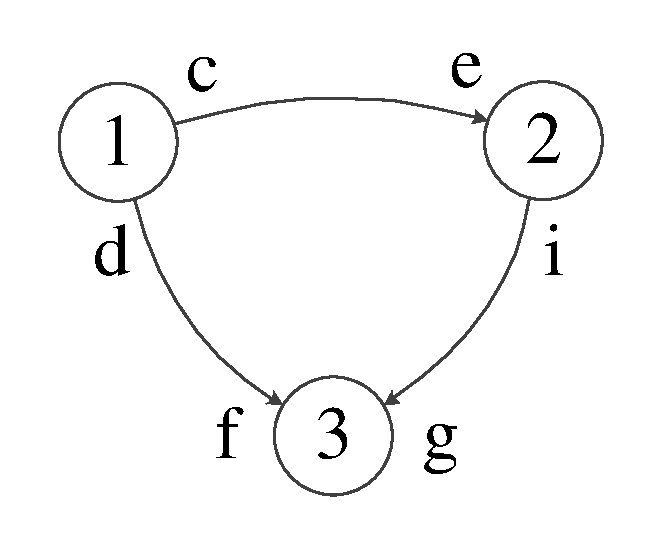
\includegraphics[height=15ex]{figure/basic-1-SDF.pdf}}}
%  {\ffigbox{\caption{SDF图中的Delay}\label{basic-SDF-Delay}}{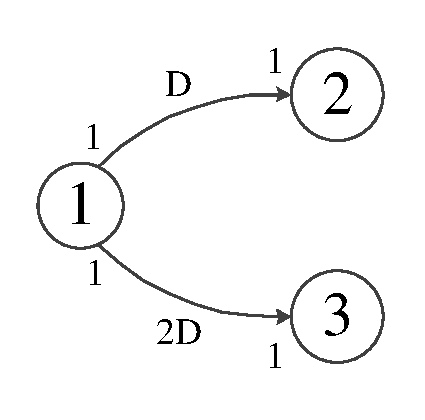
\includegraphics[height=15ex]{figure/basic-2-Delay.pdf}}}
%\end{floatrow}
%\end{figure}

图\ref{basic-SDF-sample}中从结点1到结点2的弧起点c表示结点1每运行一次在这条数据路径上产生c 单位的数据,而结点2 每运行一次在这条数据路径上消耗e 单位的数据。每个SDF 可用一个拓扑矩阵来表示,在矩阵中每列代表一个顶点,每行代表一条弧。如图\ref{basic-SDF-sample} 所示的SDF 图可由如下矩阵表示:

\begin{equation*}
  %\label{basic-SDF-matrix}
  \Gamma=\begin{bmatrix}
    c & -e & 0 \\
    d & 0 & -f \\
    0 & j & -g
  \end{bmatrix}
\end{equation*}

其中三列分别表示结点1、结点2和结点3,三行分别表示从结点1到结点2的弧、从结点1 到结点3 的弧和从结点2到结点3 的弧。由于每条弧上的两端结点运行不一定是完全同步的,因此每条弧上的数据会积累或减少,我们用向量b(n) 表示在n 时刻所有弧上的数据量,而向量

\begin{equation}
  v(n)=\begin{bmatrix}
    1 \\ 0 \\ 0
  \end{bmatrix} \textnormal{或}
  \begin{bmatrix}
    0 \\ 1 \\ 0
  \end{bmatrix} \textnormal{或}
  \begin{bmatrix}
    0 \\ 0 \\ 1
  \end{bmatrix}
\end{equation}

分别表示在n时刻运行1号结点或2号结点或3号结点。文章\cite{SDF1987} 证明了以上三者之间的关系为:

\begin{equation}
  \label{basic-eq-SDF}
  b(n+1)=b(n)+\Gamma{}v(n)
\end{equation}

弧上的Delay表示在系统开始运行前,该弧上已有多少有效数据。如图\ref{basic-SDF-Delay} 所示,在结点1 运行前,结点2 和结点3 分别可以运行1 次和2 次。

\begin{figure}[!htb]
  \centering
  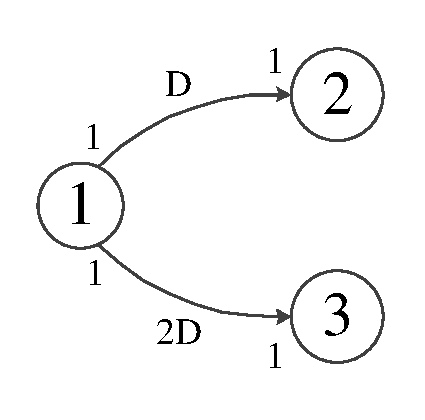
\includegraphics[height=15ex]{figure/basic-2-Delay.pdf}
  \caption{SDF图中的Delay}
  \label{basic-SDF-Delay}
\end{figure}

SDF图的Delay可以用初始时刻的b(0)向量来表示,它决定了系统可以怎样的顺序启动。如图\ref{basic-SDF-Delay} 的SDF图可以表示为

\begin{equation*}
  b(0)=\begin{bmatrix}
    1 \\ 2
  \end{bmatrix}
\end{equation*}

根据以上计算模型,假设SDF中结点数为s,文章\cite{SDF1987}证明了从SDF 图到单个处理器的一个可行的周期性串行调度(Periodic Admissible Sequential Schedule)存在的必要条件是

\begin{equation}
  \label{basic-eq-rank}
  \textnormal{rank}\Gamma=s-1
\end{equation}

由于调度是周期性的,在无限次循环的情况下,要使每条弧上的数据是一个有限值,只能使得一个周期结束后,所有弧上的数据量都回到周期开始前的状态。由\eqref{basic-eq-SDF} 式可知要满足此条件,必有

\begin{equation}
\label{basic-eq-matrix}
  \Gamma{}q=0
\end{equation}

其中向量q表示在每个周期内,每个结点的运行次数。根据以上方法,我们可以从一个SDF 图得到串行调度时每个周期内各个结点的运行次数。

但由此还无法得到一个可行的静态调度表,因为任务间有可能存在循环依赖关系。要打破循环依赖关系需要考虑将SDF转化为一个有向无环图(DAG),这要求我们首先弄清每个结点在运行时所需的数据要求哪些结点已经运行过足够的次数。假设在某SDF 图中有结点η到α的弧a,该SDF的拓扑矩阵为Γ,那么在α结点第j 次运行时,可以知道它所需的总数据量为$-j\Gamma_{a\alpha}$,弧a上原本有的数据为$b_a$,因此需要结点η 额外运行的次数为\upcite{SDF1987}

\begin{equation}
  \label{basic-eq-d}
  d_{\alpha\eta}=\left\lceil{\frac{-j\Gamma_{a\alpha}-b_a}{\Gamma{}_{a\alpha}}}\right\rceil
\end{equation}

才能够为α结点运行提供足够的数据。由以上\eqref{basic-eq-d}式可以得到从 SDF 图到 DAG 的一个S类算法\upcite{SDF1987},以解除SDF图中运算结点间的循环依赖关系。从DAG 再得到静态调度表则是NP完全问题,在运筹学上已经有所研究,目前主要用一些启发式算法,如 Hu-level 算法以及关键路径方法\upcite{HuLevel,CriticalPath}等。

此外,将任务调度到多个核上,生成静态调度表时,可以按照每个周期各结点的运行次数调度,也可按照J 个周期各结点的运行次数来调度。随着周期倍数J 的增大,得到的调度结果会越来越好。

%\emph{TODO}: 实例:一个 SDF 图的处理过程

\section{DAG调度算法简介}
\label{basic-DAG-sch}
% 简介从 DAG 到静态调度表的方法
% DLS 的主要思想

\subsection{DAG调度的分类}

从 DAG 到静态调度表的问题可分为以下四类\upcite{Comparison}:

BNP(Bounded Number of Processors):
    将 DAG 中的任务直接调度到固定个数的处理器上。处理器之间是全连接的。

UNC(Unbounded Number of Clusters):
    将 DAG 的任务调度到非限定个数的处理器上去。处理器之间是全连接的。这些算法采用的技术也称为 clustering

TDB(Task Duplication Based):
    将 DAG 的任务调度到非限定个数的处理器上去。使用任务复制技术来进一步降低完成时间。

APN(Arbitrary Processor Network):
    将任务调度到一个具有任意拓扑结构的处理器网络中去。

任务 DAG 是由一系列带有优先关系的原子任务所组成的有向无环图。一个任务结点可以有一个或多个输入,当所有输入都准备好后,该结点才可执行。在每条弧上有权重,表示从前一个任务结点到后一个任务结点的通信时间,当两个任务被分配至同一个处理器上时,该边的权重变为0。



由于我们需要考虑目标平台处理器多核之间的拓扑连接情况,而在以上四类现存算法中只有 APN 类是解决此类问题的,因此我们主要考察现存算法也主要来自这一类别。而 BNP 类算法要解决的问题是 APN 的子问题,其在解决问题的方法上有很大相似性,理解它们对解决 APN 类问题有很大帮助。

BNP 调度算法基于表调度方法。%解释表调度方法。
表调度方法中常用的图或结点的属性包括:t-level、b-level、static b-level、critical path 等\upcite{DistCompCH}:(假设$t_i$为图中的某个任务结点)% 分别解释
\begin{description}
  \item[t-level] 一个任务节点$t_i$的 t-level 属性是指从入口节点到$t_i$ (包括$t_i$) 的最长路径的长度。这里的路径长度是指这个路径上所有节点和边的权之和。
  \item[b-level] 一个节点$t_i$的b-level 属性是指从$t_i$到出口节点的最长路径的长度。所有节点的 b-level 都不会超过 DAG 的关键路径的长度。
  \item[static b-level] 一些算法在计算 b-level 的时候, 并没有考虑边权, 这样 b-level 在整个调度过程中都不会改变, 因而称为静态 b-level , 简写为SBL (Static B-Level)。
  \item[critical path] 关键路径 (Critical Path) 是一个DAG 图中最长路径。
\end{description}

BNP 中不同算法的区别主要在于针对以上属性,分配任务优先级时所采用的方法不同。有些对具有小 t-level 值的结点给与较高优先级,也有些使较大的 b-level 结点具有更高的优先级,还有些使用 b-level 与 t-level 的差值。总的来说,以 b-level 降序来调度结点,倾向于优先考虑关键路径上的任务结点;而使用 t-level 则倾向于以拓扑顺序来调度。而综合考虑 b-level 和 t-level 则产生介于以上两种情况之间的优先顺序。

    HLEFT (Highest Level First with Estimated Times)算法\upcite{HLEFT} 是一类最简单的算法,使用 static b-level 作为结点优先级。

    ISH (Insertion Scheduling Heuristic)算法\upcite{Kruatrachue1987} 将调度产生的空隙作为研究对象,向其中插入合适的任务结点。

    MCP (Modified Critical Path)算法\upcite{MCPScheduling}使用结点的 As-Last-As-Possible (ALAP) 属性作为优先级。在 CP 上的任务结点其 ALAP 值与 t-level 值相等。

    ETF (Earliest Time First)算法\upcite{ETFScheduling}每次重新计算所有可执行结点在所有处理器上的的最早开始时间来调度。

    DLS (Dynamic Level Scheduling)算法\upcite{DLS}使用 DL(Dynamic level)作为结点的优先级。DL 是结点的 static b-level 与其最早开始时间的差值。

    LAST 算法\upcite{LAST}不属于表调度算法,其主要目标是减少总的通信开销。

% 解决 DAG 问题的两种考虑 SBL 和 最早开始时间
%  DLS 的好处

APN 类算法考虑目标平台的特殊架构,如处理器数量、处理器之间的拓扑结构等。这类算法将任务调度到处理器上,并将消息传递调度到网络通信链路上,消息的调度可能取决于下层路由策略。此类中目前并没有太多算法\upcite{Comparison},下面主要讨论四种:

    MH(Mapping Heuristic)算法\upcite{MHScheduling}首先计算所有结点的 static b-level (SBL) 值,以 SBL 降序排列初始化一个 ready 结点列表,之后每个结点被调度到有最小开始时间的结点上。

    DLS(Dynamic Level Scheduling)算法\upcite{DLS},前面被分为 BNP 类算法,也可用作 APN 类算法。在用作 APN 类算法时,需要用户提供消息路由。

    BU(Bottom-Up)算法\upcite{BUScheduling} 首先寻找 DAG 的 Critical Path (CP),并将其中的所有结点都分配到同一处理器,然后将余下结点以拓扑的逆序分配给处理器,这些结点在分配时以处理器负载均衡为导向。

    BSA(Bubble Scheduling and Allocation)算法\upcite{BSA}以增量的方式逐渐形成一个优化的调度结果。首先将所有结点分配到一个枢轴处理器上(连接最多的处理器),然后算法试着将结点移到临近处理器上以提高每个结点的开始时间。枢轴处理器上所有结点都处理过后,将下一个处理器作为新的枢轴处理器。整个过程以宽度优先变换枢轴处理器不断重复,直到没有结点可被提前。

\subsection{DLS算法简介}
\label{basic-DLS-intro}

Dynamic Level Scheduling (DLS)算法\upcite{DLS}使用了一个动态层次 DL (Dynamic Level)作为任务调度排序的指标。DL 是一个结点的静态层数(SBL) 与它在一个处理器上的最早开始时间之差,相当于综合考虑了CP上的任务和 能够早开始的任务可以尽早开始 两方面情况。在调度的每个步骤中,算法要对在就绪池中的每个结点,计算它们在所有处理器上的 DL。 具有最大 DL 的结点-处理器对被挑选出来进行调度。其中在考虑各个任务于每个处理器上的最早开始时间时,需要根据下层路由得到消息在链路上的调度情况。

DLS算法的步骤如算法\ref{algo-DLS}所述,它的时间复杂度为 $O(n^{2}p f(p))$,其中$n$为 DAG 中的结点个数,$p$为处理器个数,$f(p)$是消息路由算法的时间复杂度。
% 待修改为算法格式
%\begin{Verbatim}[numbers=left,frame=single,xleftmargin=50pt]
%    (1)计算每个结点的 b-level 值
%    (2)初始化就绪结点池,使之包含所有入口结点。
%    反复执行以下步骤,直到所有结点调度完毕:
%        (2.1)计算每个结点在每个处理器上的最早开始时间,再将结点
%        的 SBL 减去最早开始时间,即计算出每个(结点-处理器)对的 DL
%        (2.2)选择具有最大 DL 的结点-处理器对,将该结点调度到相应
%        处理器上
%        (2.3)将最近的就绪结点加入到就绪池中
%\end{Verbatim}

\begin{algorithm}
\caption{DLS 算法}
\label{algo-DLS}
\KwIn{DAG 任务图,目标处理器平台}
\KwOut{静态调度表}
计算 DAG 中每个结点的 b-level 值 (SBL)\;
初始化就绪结点池 R,使之包含所有入口结点\;
\While{R 不空}{
    计算 R 中每个结点在每个处理器上的最早开始时间,再将结点的 SBL 减去最早开始时间,即计算出每个(结点-处理器)对的 DL\;
    选择具有最大 DL 的(结点-处理器)对,将该结点调度到相应处理器上\;
    将新的就绪结点加入到就绪池 R 中\;
}
\end{algorithm}


\section{分区系统简介}
\label{basic-partition}

在分区操作系统中,各个分区之间应该相互隔离,分区应为应用提供时间分区与空间分区。应用运行在系统为其提供的分区环境中,不受其他分区的影响。分区是分区操作系统分配资源的单位。

\subsection{分区、任务与处理器的关系}
% 以下几段来自赵纯毕设,最终提交前要改
分区的时间资源是指各个分区获得的处理器使用时间。运行于同一处理器上的所有分区共享此处理器的计算资源。分区系统需要保证分区能够获得固定的时间进而获得处理器的计算能力。操作系统以分区为单位分配处理器资源,在操作系统分配处理器资源时,并不感知分区内部的任务,即使一个分区内部不存在任务,那么操作系统也会将此处理器资源分配给相应分区,而不是分配给其他分区。同分区内的所有任务根据分区内任务调度算法共享分区的时间资源。分区系统需要保证分区不会使用其他分区的时间资源,这样系统能够保证分区的时间隔离。

分区空间资源是每个分区所有的地址空间。空间资源包括内存资源,I/O资源等。内存资源包括分区能够访问的虚拟地址空间和物理内存空间等,其中I/O资源包括分区能够访问的I/O 设备以及共享I/O设备中获得的带宽。空间资源由操作系统以分区为单位分配,分区间无共享资源,而分区内部的任务共享本分区内空间资源。

根据 ARINC 653 标准中关于分区与任务间关系的定义,分区是资源的分配单位,任务是系统的调度单位。应用通过任务来实现具体的功能操作,而分区为任务提供具体的分区环境与所需资源。一个分区内部可以有一个或者多个任务,而一个任务只能属于一个分区。

在分区与处理器的关系方面,ARINC 653 标准规定一个分区只能运行于一个处理器上,不允许分区在处理器之间迁移。分区与处理器之间的关系如图 \ref{basic-fig-partition} 所示。

\begin{figure}[!hbt]
  \centering
  % Requires \usepackage{graphicx}
  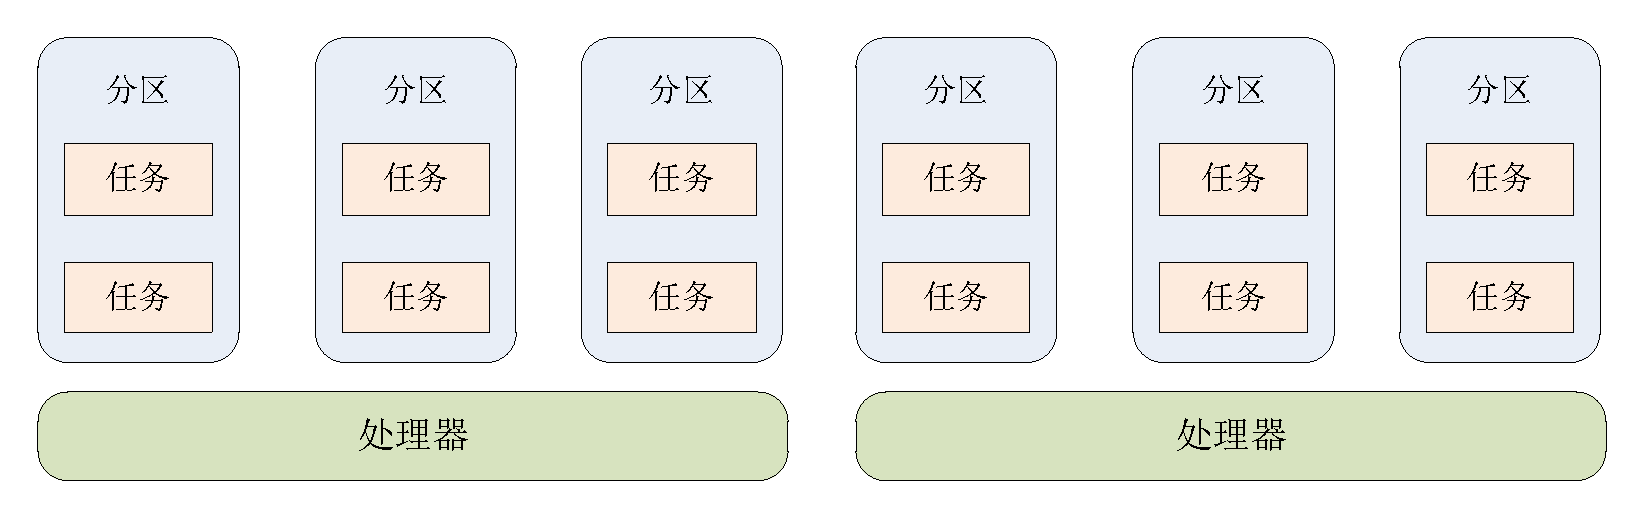
\includegraphics[height=25ex]{figure/basic-partition.pdf}\\
  \caption{分区与处理器的关系}\label{basic-fig-partition}
\end{figure}

\subsection{分区与任务调度的关系}

分区通过时间和空间两方面来实现,其中时间分区通过为各分区分配不同的处理器时间来实现,因此时间分区与调度系统直接相关。分区系统的调度通常分为两层,上层是处理器针对运行在其上的分区间调度,下层是各分区内部任务间的调度,两层可以各采用不同的调度策略。其中分区间调度可以是周期性的,也可以是非周期的,如果我们确切已知每个分区内部任务所需的总运行时间,则只需给每个分区分配其所需时间即可。

本文采用的是静态调度算法,在任务调度前即可知道任务数量、所有任务的时间信息等,因此可以根据任务属性,将所有任务均以分区隔离,每个分区内仅分配一个任务,使得任务与分区一一对应。这样即可使下层的分区内调度非常简单,分区内仅有一个任务,分区的运行时间即是分区内任务的运行时间。而上层调度所面对的各分区的时间属性与其内部所运行任务的时间属性相一致,因此上层针对分区的调度亦可认为是直接面向任务的调度,只需根据对应任务的时间属性分配即可。

\subsection{分区间通信}
\label{basic-partition-message}

处理器或核间通信可采用总线共享 Cache 或共享内存的方式来实现,也可采用片上互连的方式,如交叉开关或片上网络等。本文假定处理器或多核之间是基于片上互连的方案,各个处理器核心之间通过消息通信,其通信时间直接与通信数据量相关。如果核间消息传递速率为 s (即单位时间传递 s 的数据量),则传递 M 的数据需要 $M/s$ 的时间延迟。核间消息的传递是双向的,且同一个核可同时与多个与其有直接链路相连的核进行通信互不影响。

由于一个处理器或核上可以有多个分区,因此分区间通信包含同处理器上与不同处理器上的两种情况。同处理器上的分区间通信可直接通过缓存或共享内存来实现,本文假定其延时很小可忽略;而不同处理器上的分区之间通信则须采用处理器或核间通信的方式,如上段所述有一定延迟,并在此期间占用相应链路上的通信资源。

\section{本章小结}

本章主要介绍了与论文相关的理论与技术。首先对周期性与偶发实时任务模型的相关调度算法理论做了简单总结,从任务模型、时间约束、调度环境、单处理器及多处理器调度等方面做了讨论。其次介绍了多核平台下的几种计算模型及其各自的特点,并着重介绍了SDF 模型,这是论文中所述算法的切入点,然后简要介绍了从 SDF 图转化为 DAG 的一种 S 类算法。本章还介绍了从 DAG 生成静态调度表的现有算法分类,所解决的问题类型以及各自的特点,并着重介绍了可用于 APN 问题的 DLS 算法,它是从 DAG 得到最终的静态调度表的算法基础。本章最后对分区操作系统中的任务与分区的相关概念做了介绍。

